\documentclass[a4paper,12pt]{article}
\usepackage[hmargin=2.5cm,vmargin=2.5cm]{geometry}

\usepackage[utf8]{inputenc}   % le fichier .tex est en UTF-8     
\usepackage[francais]{babel}  %typo française                    
\usepackage[T1]{fontenc}      % encodage des fonts latex         
\usepackage{lmodern}                                             
\usepackage{microtype}        % typo supplémentaires             


\usepackage{multirow}  %  pour des tableaux multilignes/multicolonnes

\usepackage{graphicx} %inclusion de graphiques

\usepackage{hyperref} % liens dans le pdf
\hypersetup{%
  pdftitle={Title},
  pdfauthor={Author1, Author2},
  pdfkeywords={keywords}
  pdfsubject={article},
  colorlinks=true,
  linkcolor=black,
  urlcolor=black,
  citecolor=black
}




\begin{document}

   \section{Les protocoles} 



   \subsection{Les protocoles Monte Carlo} 
    
    \begin{table}[!htbp]
      \centering

      \begin{tabular}{|l|r|r|c|c|}

        \hline
        Nom & Temp & Traj (mega)& seuil voisin  & Proba \\
        \hline
        MC0   & 0.01  &  6000 & 0 & 0; 1; 0.1; 0   \\  
        MC0-  & 0.01  &   300 & 0 & 0; 1; 0.1; 0   \\  
        MC4   & 0.2   &  6000 & 0 & 0; 1; 0.1; 0   \\          
        MC4-  & 0.2   &   300 & 0 & 0; 1; 0.1; 0   \\ 
        MC42  & 0.2   &  6000 & 0 & 1; 0; 0.1; 0   \\        
        MC42- & 0.2   &   300 & 0 & 1; 0; 0.1; 0   \\   \hline                   

       
      \end{tabular}      
      \caption{Les protocoles Monte Carlo}
      \label{tab_protoMC}      
    \end{table}

   \subsection{Les protocoles Replica Exchange} 
    
    \begin{table}[!htbp]
      \centering

      \begin{tabular}{|l|l|r|r|r|c|c|}

        \hline
        Nom & marcheurs &Temp & Traj (mega)& seuil voisin  & Proba & swap period (mega)\\
        \hline
        RE1   & 4 & 10<->0.01    &  1500 & 10 & 1; 0; 0.1; 0 &  7.5\\  
        RE2   & 4 & 1<->0.125    &  1500 & 10 & 1; 0; 0.1; 0 &  7.5\\  
        RE2-  & 4 & 1<->0.125    &  250  & 10 & 1; 0; 0.1; 0 &  2.5\\  
        RE22  & 4 & 2<->0.25     &  1500 & 10 & 1; 0; 0.1; 0 &  7.5\\  
        RE3   & 8 & 3<->0.175    &  750  & 10 & 1; 0; 0.1; 0 &  7.5\\
        RE32  & 8 & 3<->0.175    &  750  & 10 & 0; 1; 0.1; 0 &  7.5\\
        RE4   & 8 & 10<->0.00316 &  750  & 10 & 1; 0; 0.1; 0 &  1\\  
        RE42  & 8 & 10<->0.00316 &  750  &  0 & 1; 0; 0.1; 0 &  2.5\\  \hline

      \end{tabular}      
      \caption{Les protocoles Replica Exchange}
      \label{tab_protoRE}      
    \end{table}


   \subsection{Les protocoles Heuristic} 
    
    \begin{table}[!htbp]
      \centering

      \begin{tabular}{|c|r|}

        \hline
        Nom & nombre de cycles \\
        \hline
        h   & 110000 \\  
        h-  & 1100   \\  \hline

      \end{tabular}      
      \caption{Les protocoles Heuristic}
      \label{tab_protoH}      
    \end{table}

   \section{Tous les résidus actifs} 

   \subsection{Les temps de calculs} 

    \begin{table}[!htbp]
      \centering

      \begin{tabular}{|c|c|c|c|c|c|c|c|c|}

 
        \hline
        & h & MC3 & MC43 & RE1 & RE2 & RE5 & RE3 & RE4 \\
        \hline
        1A81 & 20:19:08 & 8:29:23 & 9:41:15 & 4:14:08 & 2:31:33 & 4:12:24 & 3:39:51 & 4:49:59 \\
        1ABO & 4:46:51 & 3:09:21 & 3:16:33 & 2:58:01 & 1:27:50 & 3:06:43 & 2:02:08 & 1:50:16 \\
        1BM2 & 17:57:45 & 8:08:43 & 8:38:39 & 5:04:51 & 3:05:15 & 4:10:46 & 3:31:43 & 3:09:45 \\
        1CKA & 5:51:19 & 3:15:59 & 3:24:43 & 2:25:53 & 1:27:11 & 2:32:08 & 2:05:03 & 2:06:42 \\
        1G9O & 12:15:20 & 5:51:24 & 6:15:08 & 3:44:15 & 2:12:23 & 4:29:59 & 3:05:30 & 2:46:02 \\
        1M61 & 18:12:19 & 7:41:35 & 8:07:18 & 3:55:23 & 2:20:05 & 4:07:41 & 3:14:59 & 3:30:48 \\
        1O4C & 21:42:26 & 9:08:38 & 9:57:44 & 4:44:12 & 2:46:47 & 4:27:51 & 4:34:02 & 3:29:06 \\
        1R6J & 12:15:27 & 5:32:21 & 5:59:11 & 3:25:07 & 2:07:39 & 3:27:18 & 3:34:57 & 2:45:59 \\
        2BYG & 15:08:07 & 6:28:44 & 6:56:15 & 3:50:38 & 2:52:42 & 4:49:02 & 3:58:10 & 2:56:50 \\

\hline

      \end{tabular}      
      \caption{les temps de calculs (hh:mm:ss) pour tous les résidus actifs}
      \label{tab_temps_all}      
    \end{table}


   \subsection{Les meilleures énergies} 

    \begin{table}[!htbp]
      \centering

      \begin{tabular}{|c|c|c|c|c|c|c|c|c|c|}

        \hline
        Protéine & h & MC3 & MC43 & RE1 & RE2 & RE5 & RE3 & RE32 & RE4 \\
        \hline
        1A81 & -521 & -538 & -522 & -525 & -520 & -520 & -514 & -512 & -518 \\
        1ABO & -272 & -274 & -268 & -273 & -269 & -273 & -268 & -271 & -272 \\
        1BM2 & -484 & -500 & -486 & -488 & -481 & -489 & -478 & -476 & -486 \\
        1CKA & -252 & -258 & -249 & -259 & -251 & -251 & -247 & -246 & -249 \\
        1G9O & -428 & -435 & -428 & -429 & -421 & -430 & -428 & -425 & -428 \\
        1M61 & -480 & -493 & -479 & -483 & -480 & -481 & -480 & -480 & -480 \\
        1O4C & -535 & -545 & -531 & -536 & -529 & -536 & -527 & -524 & -532 \\
        1R6J & -407 & -419 & -414 & -415 & -409 & -411 & -409 & -408 & -414 \\
        2BYG & -457 & -469 & -454 & -461 & -456 & -460 & -456 & -454 & -462 \\
        
        \hline

      \end{tabular}      
      \caption{les meilleurs énergies pour tous les résidus actifs}
      \label{tab_best_ener_all}      
    \end{table}


   \begin{figure}[t]
     \centering
     \begin{tabular}{cc}
       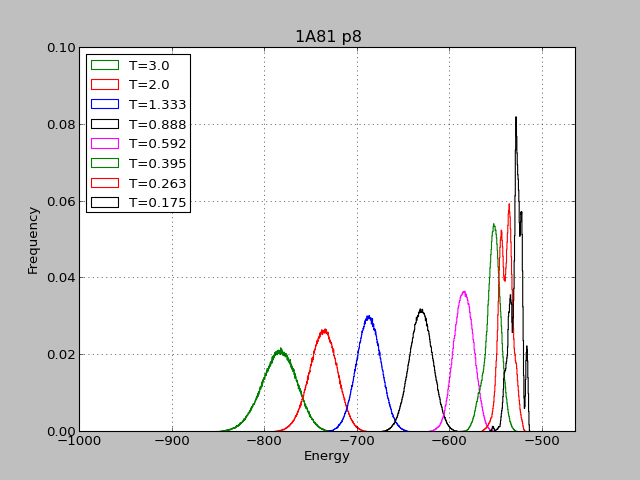
\includegraphics[width=12cm]{image/1A81_casa-p8.png} &
     \end{tabular}
     
     \caption{Distribution des énergies selon la température (protocole RE3).}
     \label{Distrib_E_RE3}
   \end{figure}



   \begin{figure}[t]
     \centering
     \begin{tabular}{cc}
       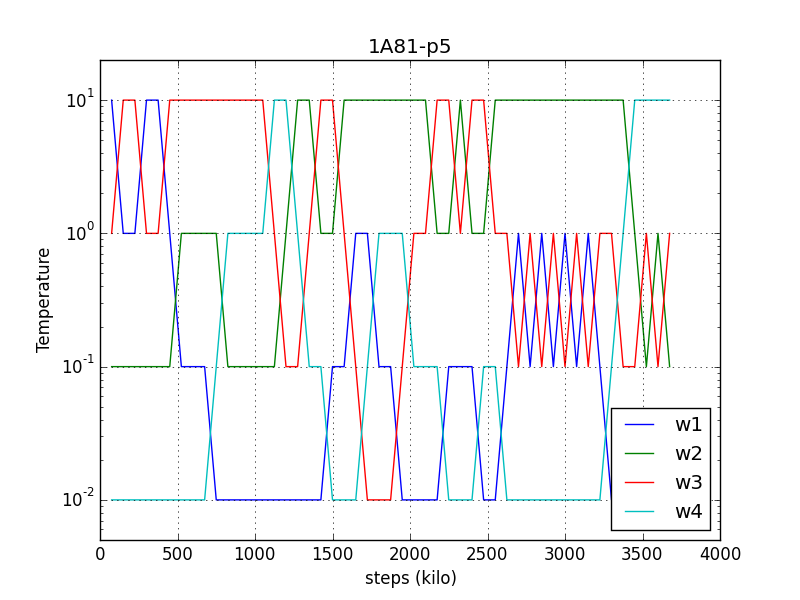
\includegraphics[width=12cm]{image/1A81-p5-T_traj.png} &
     \end{tabular}
     
     \caption{Variation de la température au court de la trajectoire de chaque marcheur (protocole RE1).}
     \label{TRAJ_T_RE1}
   \end{figure}

   \section{Avec des résidus gélés}
 
   \subsection{Séquence native}


    \begin{table}[!htbp]
      \centering

      \begin{tabular}{|c|c|c|c|c|c|c|}

        \hline
        Protéine & GMEC & H- & MC0 & MC4- \\
        \hline
        1A81 & -585.1365 & 0 & .2547 & 0 \\
        1ABO & -320.1798 & 0 & 0 & 0 \\
        1BM2 & -553.5532 & 0 & .0564 & .0121 \\
        1CKA & -319.2787 & 0 & 0 & 0 \\
        1G9O & -481.1175 & 0 & .1394 & 0 \\
        1M61 & -555.9140 & 0 & 0 & 0 \\
        1O4C & -591.2115 & 0 & 0 & .1250 \\
        1R6J & -454.9340 & 0 & 0 & 0 \\
        2BYG & -507.0165 & 0 & 0 & 0 \\        
        \hline




      \end{tabular}      
      \caption{l'énergie du GMEC et la différence avec les autres protocoles.Tous les résidus sont gélés}
      \label{tab_best_ener_no_active}      
    \end{table}

   \subsection{Séquence native}


    \begin{table}[!htbp]
      \centering

      \begin{tabular}{|c|c|c|c|c|c|c|}

        \hline
        Protéine & GMEC & H- & MC0 & MC4- \\
        \hline
        1A81 & -585.1365 & 0 & .2547 & 0 \\
        1ABO & -320.1798 & 0 & 0 & 0 \\
        1BM2 & -553.5532 & 0 & .0564 & .0121 \\
        1CKA & -319.2787 & 0 & 0 & 0 \\
        1G9O & -481.1175 & 0 & .1394 & 0 \\
        1M61 & -555.9140 & 0 & 0 & 0 \\
        1O4C & -591.2115 & 0 & 0 & .1250 \\
        1R6J & -454.9340 & 0 & 0 & 0 \\
        2BYG & -507.0165 & 0 & 0 & 0 \\        
        \hline


      \end{tabular}      
      \caption{l'énergie du GMEC et la différence avec les autres protocoles.Tous les résidus sont gélés}
      \label{tab_best_ener_no_active}      
    \end{table}


   \subsection{ Une position active}


    \begin{table}[!htbp]
      \centering

      \begin{tabular}{|c|c|c|}


        \hline
        Position & GMEC & MC4- \\
        \hline
        14 & -584.4693 & .0405 \\
        39 & -584.7378 & .0111 \\
        55 & -584.0477 & .0012 \\
        60 & -583.7763 & .0140 \\
        66 & -592.3835 & .0347 \\
        70 & -583.8950 & .0348 \\
        71 & -588.5916 & .0247 \\
        76 & -583.3815 & .0248 \\
        79 & -582.8485 & .0406 \\
        86 & -584.1412 & .0248 \\
        101 & -583.8406 & .0248 \\
        105 & -583.0197 & .0248 \\
        107 & -582.2241 & .0248 \\

        \hline


      \end{tabular}      
      \caption{Liste des echecs pour 1A81}
      \label{tab_best_ener_no_active}      
    \end{table}


    \begin{table}[!htbp]
      \centering

      \begin{tabular}{|c|c|c|}


        \hline
        Position & GMEC & MC4- \\
        \hline
        2 & -553.3134 & .0040 \\
        3 & -553.5532 & .0121 \\
        5 & -553.0932 & .0179 \\
        6 & -553.5532 & .0121 \\
        8 & -556.1917 & .0148 \\
        10 & -551.4990 & .0149 \\
        11 & -551.8859 & .0149 \\
        12 & -550.8152 & .0148 \\
        13 & -553.4829 & .0451 \\
        14 & -553.5532 & .0121 \\
        15 & -553.5532 & .0121 \\
        17 & -553.5532 & .0121 \\
        18 & -553.0880 & .0121 \\
        19 & -553.5532 & .0270 \\
        20 & -553.0003 & .0121 \\
        21 & -553.5532 & .0121 \\
        22 & -553.1769 & .0121 \\
        29 & -553.5532 & .0121 \\
        34 & -553.5532 & .0270 \\
        36 & -555.3358 & .0317 \\
        37 & -553.5532 & .0121 \\
        41 & -553.5076 & .0121 \\
        46 & -552.9056 & .0149 \\
        49 & -553.5532 & .0121 \\
        51 & -553.5532 & .0179 \\
        55 & -551.8384 & .0121 \\
        56 & -553.5532 & .0121 \\
        57 & -561.0695 & .0121 \\
        58 & -553.5532 & .0121 \\
        62 & -553.5532 & .0121 \\
        65 & -553.5532 & .0121 \\
        66 & -551.2026 & .0179 \\
        68 & -552.6182 & .0148 \\
        70 & -553.5532 & .0121 \\
        72 & -552.2724 & .0121 \\
        73 & -553.5532 & .0121 \\
        75 & -553.5532 & .0179 \\
        77 & -553.0234 & .0466 \\
        80 & -553.5532 & .0121 \\
        81 & -553.5532 & .0121 \\
        82 & -548.0641 & .0121 \\
        83 & -553.5532 & .0121 \\
        85 & -550.1884 & .0122 \\
        86 & -552.7375 & .0148 \\
        87 & -550.6139 & .0121 \\
        90 & -552.8601 & .0009 \\
        91 & -553.5532 & .0121 \\
        92 & -553.5532 & .0121 \\
        93 & -553.2772 & .0148 \\
        94 & -553.3207 & .0251 \\
        96 & -553.5532 & .0121 \\
        \hline


      \end{tabular}      
      \caption{Liste des echecs pour 1BM2}
      \label{tab_best_ener_no_active}      
    \end{table}




    \begin{table}[!htbp]
      \centering

      \begin{tabular}{|c|c|c|}


        \hline
        Position & GMEC & MC4- \\
        \hline
        17 & -316.1693 & .0109 \\

\hline
      \end{tabular}      
      \caption{Liste des echecs pour 1CKA}
      \label{tab_echec_1CKA_1}      
    \end{table}

    \begin{table}[!htbp]
      \centering

      \begin{tabular}{|c|c|c|}

        \hline
        \hline
        Position & GMEC & MC4 \\
        \hline
        58 & -561.9469 & .0138 \\
        
        \hline

      \end{tabular}      
      \caption{Liste des echecs pour 1M61}
      \label{tab_echec1M61__1}      
    \end{table}
    

    \begin{table}[!htbp]
      \centering
      
      \begin{tabular}{|c|c|c|}
        



        \hline
        Position & GMEC & MC4- \\
        \hline
        1 & -591.2115 & .1380 \\
        2 & -591.2115 & .1250 \\
        3 & -591.2115 & .1250 \\
        4 & -590.7216 & .0319 \\
        5 & -590.5458 & .1071 \\
        6 & -591.2115 & .1521 \\
        7 & -590.7923 & .1429 \\
        8 & -591.2115 & .1250 \\
        9 & -591.2115 & .1728 \\
        10 & -591.2115 & .2572 \\
        11 & -589.9443 & .2489 \\
        12 & -591.1022 & .1137 \\
        13 & -589.9867 & .0535 \\
        14 & -591.2115 & .1250 \\
        15 & -589.4899 & .0436 \\
        16 & -591.2115 & .1521 \\
        17 & -590.4460 & .0557 \\
        18 & -589.0053 & .1366 \\
        19 & -590.7580 & .0348 \\
        20 & -591.2115 & .1250 \\
        21 & -591.2115 & .1600 \\
        22 & -591.2115 & .1250 \\
        23 & -590.5249 & .1530 \\
        24 & -590.7262 & .0630 \\
        25 & -591.2115 & .1250 \\
        26 & -591.2115 & .1250 \\
        27 & -590.8058 & .1194 \\
        28 & -591.2115 & .1250 \\
        29 & -591.2115 & .1571 \\
        30 & -590.5207 & .0221 \\
        31 & -590.5507 & .0530 \\
        32 & -591.2115 & .1571 \\
        33 & -591.2115 & .1234 \\
        34 & -590.7486 & .1258 \\
        35 & -591.2115 & .0378 \\
        36 & -589.1510 & .0974 \\
        37 & -591.0133 & .0941 \\
        38 & -589.2126 & .2743 \\
        39 & -589.0387 & .1890 \\
        40 & -590.8793 & .0883 \\
        41 & -589.4209 & .0409 \\
        42 & -591.2115 & .1250 \\
        43 & -587.9420 & .1315 \\
        44 & -589.8470 & .0595 \\
        45 & -591.2115 & .1712 \\
        46 & -588.8346 & .2668 \\
        47 & -589.9117 & .2773 \\
        48 & -588.6520 & .2625 \\
        49 & -591.2115 & .2120 \\
        50 & -590.6561 & .0807 \\
        51 & -591.1249 & .2986 \\
        52 & -589.7127 & .2734 \\
        53 & -590.7224 & .3012 \\
        54 & -590.8735 & .3615 \\
        55 & -588.6242 & .2007 \\
        56 & -591.2115 & .2120 \\
        57 & -591.2115 & .1250 \\
        58 & -590.6832 & .0743 \\
        59 & -591.2115 & .0378 \\
        60 & -591.1842 & .1082 \\
        61 & -590.6996 & .1272 \\
        62 & -595.8620 & .0899  \\
        63 & -591.2115 & .0974 \\
        64 & -588.8836 & .1014 \\
        65 & -591.2115 & .1571 \\
        66 & -590.1420 & .1533 \\
        67 & -587.5415 & .0433 \\
        68 & -590.1771 & .1541 \\
        69 & -591.2115 & .1250 \\
        70 & -590.4684 & .1066 \\
        71 & -591.2115 & .1250 \\
        72 & -591.2115 & .1311 \\
        73 & -591.2115 & .1250 \\
        74 & -588.7096 & .1169 \\
        75 & -590.2437 & .0505 \\
        76 & -591.2115 & .1521 \\
        78 & -587.6940 & .0821 \\
        79 & -589.9770 & .1380 \\
        80 & -591.1165 & .0661 \\
        81 & -590.2528 & .1229 \\
        82 & -589.8459 & .0724 \\
        83 & -590.2079 & .0513 \\
        84 & -591.2095 & .0433 \\
        85 & -590.8011 & .1154 \\
        87 & -590.7787 & .0744 \\
        88 & -590.2860 & .0857 \\
        89 & -591.2115 & .1250 \\
        90 & -590.2493 & .1084 \\
        91 & -589.5602 & .0694 \\
        92 & -589.3260 & .1838 \\
        93 & -590.4697 & .0188 \\
        94 & -587.4192 & .3392 \\
        95 & -590.0201 & .2937 \\
        96 & -590.6312 & .2723 \\
        97 & -595.0049 & .2864 \\
        98 & -590.0135 & .2013 \\
        99 & -589.7855 & .2932 \\
        100 & -591.2115 & .2120 \\
        101 & -591.2115 & .2120 \\
        102 & -591.2115 & .2572 \\
        103 & -595.4168 & .1277 \\
        104 & -589.9208 & .3581 \\
        
        \hline


      \end{tabular}      
      \caption{Liste des echecs pour 1O4C}
      \label{tab_echec1O4C__1}      
    \end{table}

    \begin{table}[!htbp]
      \centering

      \begin{tabular}{|c|c|c|}


        \hline
        Position & GMEC & MC4- \\
        \hline
         4 & -453.4484 & .0155  \\
        20 & -452.6464 & .0114 \\
        32 & -454.9340 & .0092 \\
        68 & -454.4856 & .0060 \\
        73 & -454.7809 & .0155 \\
        77 & -454.1344 & .0155 \\
        79 & -453.4729 & .0155 \\
        
        \hline


      \end{tabular}      
      \caption{Liste des echecs pour 1R6J }
      \label{tab_echec1R6J__1}      
    \end{table}


    \begin{table}[!htbp]
      \centering

      \begin{tabular}{|c|c|c|}

        \hline
        Position & GMEC & MC4- \\
        \hline
        1 & -505.2910 & .0132 \\
        3 & -506.7960 & .0254 \\
        4 & -505.5800 & .0023 \\
        5 & -506.8732 & .0948 \\
        49 & -505.5183 & .0135 \\
        59 & -507.0165 & .0100 \\
        85 & -506.6217 & .0101 \\
        88 & -505.2286 & .0097 \\
        95 & -506.3195 & .0131 \\

        \hline


      \end{tabular}      
      \caption{Liste des echecs pour 2BYG }
      \label{tab_echec2BYG__1}      
    \end{table}


   \subsection{ Cinq positions actives}


    \begin{table}[!htbp]
      \centering

      \begin{tabular}{|c|c|c|c|}



   \hline
   \hline
   Protéine & GMEC & H & MC4 \\
   \hline
   1A81 1 & -579.3989 & 0 & 0 \\
   1A81 2 & -575.2254 & 0 & 0 \\
   1A81 3 & -582.7452 & 0 & 0 \\
   1A81 4 & -569.9383 & 0 & 5.3443 \\
   1A81 5 & -591.8143 & 0 & 0 \\
   1ABO 1 & -315.4497 & 0 & 0 \\
   1ABO 2 & -316.6637 & 0 & 0 \\
   1ABO 3 & -307.4824 & 0 & 0 \\
   1ABO 4 & -313.7710 & 0 & 0 \\
   1ABO 5 & -313.5695 & 0 & 0 \\
   1BM2 1 & -548.2341 & 0 & 0 \\
   1BM2 2 & -554.8135 & 0 & 0 \\
   1BM2 3 & -557.8629 & 0 & 0 \\
   1BM2 4 & -544.9791 & 0 & 0 \\
   1BM2 5 & -550.2956 & 0 & .0121 \\
   1CKA 1 & -315.0859 & 0 & 0 \\
   1CKA 2 & -309.7692 & 0 & 0 \\
   1CKA 3 & -317.3820 & 0 & 0 \\
   1CKA 4 & -314.8550 & 0 & 0 \\
   1CKA 5 & -312.0405 & -.0001 & -.0001 \\
   1G9O 1 & -469.9540 & 0 & 0 \\
   1G9O 2 & -476.4094 & 0 & 0 \\
   1G9O 3 & -479.7190 & 0 & 0 \\
   1G9O 4 & -478.9513 & 0 & 0 \\
   1G9O 5 & -480.7260 & 0 & 0 \\
   1M61 1 & -557.6647 & 0 & 0 \\
   1M61 2 & -546.9587 & 0 & 0 \\
   1M61 3 & -553.0731 & 0 & 0 \\
   1M61 4 & -555.0885 & 0 & 0 \\
   1M61 5 & -554.6356 & 0 & 0 \\
   1O4C 1 & -584.4267 & 0 & .0655 \\
   1O4C 2 & -584.8989 & 0 & .1437 \\
   1O4C 3 & -588.4971 & 0 & .1164 \\
   1O4C 4 & -587.7129 & 0 & .1400 \\
   1O4C 5 & -587.6514 & 0 & .1168 \\
   1R6J 1 & -444.5018 & 0 & 0 \\
   1R6J 2 & -449.3043 & 0 & .9421 \\
   1R6J 3 & -453.1139 & 0 & 0 \\
   1R6J 4 & -453.1139 & 0 & 0 \\
   1R6J 5 & -454.9340 & 0 & 0 \\
   2BYG 1 & -500.7946 & 0 & .0150 \\
   2BYG 2 & -506.2319 & 0 & 0 \\
   2BYG 3 & -506.8744 & 0 & .0131 \\
   2BYG 4 & -504.5135 & 0 & 0 \\
   2BYG 5 & -506.0052 & 0 & 0 \\
   
   \hline

 \end{tabular}      
 \caption{Liste des echecs pour 2BYG }
 \label{tab_echec2BYG__1}      
\end{table}


   \subsection{ Dix positions actives}


    \begin{table}[!htbp]
      \centering

      \begin{tabular}{|c|c|c|c|}

        \hline
        Protéine & GMEC & H & MC4 \\
        \hline
        1A81 1 & -583.9354 & 0 & 0 \\
        1A81 2 & -581.7802 & 0 & 0 \\
        1A81 3 & -587.4392 & .0001 & .1595 \\
        1A81 4 & -589.1322 & 0 & .0317 \\
        1A81 5 & -578.2558 & 0 & .0563 \\
        1ABO 1 & -309.1670 & .0675 & .9054 \\
        1ABO 2 & -308.8387 & 0 & 0 \\
        1ABO 3 & -303.8520 & 0 & 0 \\
        1ABO 4 & -310.0087 & 0 & .0128 \\
        1ABO 5 & -301.6727 & 0 & 0 \\
        1BM2 1 & -549.8638 & 0 & .0950 \\
        1BM2 2 & -541.5944 & 0 & 0 \\
        1BM2 3 & -543.7434 & 0 & 0 \\
        1BM2 4 & -549.0453 & 0 & 0 \\
        1BM2 5 & -544.1447 & 0 & .1082 \\
        1CKA 1 & -305.8477 & 0 & 0 \\
        1CKA 2 & -309.9886 & 0 & 0 \\
        1CKA 3 & -304.6618 & 0 & 0 \\
        1CKA 4 & -302.4894 & 0 & 0 \\
        1CKA 5 & -299.2329 & .2859 & 3.2525 \\
        1G9O 1 & -466.6764 & 0 & 0 \\
        1G9O 2 & -478.8797 & 0 & 0 \\
        1G9O 3 & -477.2503 & .1366 & 0 \\
        1G9O 4 & -470.6458 & 0 & 0 \\
        1G9O 5 & -464.8659 & 0 & 3.9599 \\
        1M61 1 & -550.0699 & 0 & .0776 \\
        1M61 2 & -538.6026 & 3.5105 & 4.5062 \\
        1M61 3 & -552.2673 & 0 & 0 \\
        1M61 4 & -550.0553 & 0 & 0 \\
        1M61 5 & -553.6559 & 0 & .0432 \\
        1O4C 1 & -587.4665 & 0 & .1121 \\
        1O4C 2 & -585.8545 & 0 & .1046 \\
        1O4C 3 & -580.3505 & 0 & .1519 \\
        1O4C 4 & -587.1548 & 0 & .1545 \\
        1O4C 5 & -590.2650 & 0 & .1753 \\
        1R6J 1 & -448.8351 & 0 & 2.4022 \\
        1R6J 2 & -448.4631 & 0 & 1.0398 \\
        1R6J 3 & -450.3950 & 0 & .0106 \\
        1R6J 4 & -451.7211 & 0 & 0 \\
        1R6J 5 & -450.9943 & 0 & .0162 \\
        2BYG 1 & -511.3882 & -5.7485 & -5.7148 \\
        2BYG 2 & -504.7389 & 0 & 0 \\
        2BYG 3 & -504.3048 & 0 & .0833 \\
        2BYG 4 & -504.3466 & 0 & .2149 \\
        2BYG 5 & -491.6095 & 0 & 0 \\

        \hline


 \end{tabular}      
 \caption{Résultats 10 positions actives }
 \label{tab_echec2BYG__1}      
\end{table}


   \subsection{ Vingt positions actives}


    \begin{table}[!htbp]
      \centering

      \begin{tabular}{|c|c|c|c|}


        \hline
        Protéine & GMEC & H & MC4 \\
        \hline
        1A81 1 & -566.9106 & 0 & .3275 \\
        1A81 2 & -564.6618 & .1705 & 2.4355 \\
        1A81 3 & -572.9780 & 0 & .4640 \\
        1A81 4 & -572.9780 & .3568 & .5088 \\
        1A81 5 & -572.9780 & .3568 & .5088 \\
        1ABO 1 & -299.6592 & .1205 & 1.1159 \\
        1ABO 2 & no & -298.3854 & -298.3854 \\
        1ABO 3 & no & -298.3854 & 298.3854 \\
        1ABO 4 & no & -297.8545 & -297.8621 \\
        1ABO 5 & no & -297.8009 & -298.7492 \\
        1BM2 1 & -526.0936 & 0 & .0619 \\
        1BM2 2 & no & -525.3588 & -525.4313 \\
        1BM2 3 & -534.3860 & .0230 & .4763 \\
        1BM2 4 & no & -526.8307 & -529.4190 \\
        1BM2 5 & -535.3334 & .2396 & .3746\\
        1CKA 1 & -295.8571 & 0 & 0 \\
        1CKA 2 & -295.8571 & 0 & 0 \\
        1CKA 3 & -293.8687 & 0 & 0 \\
        1CKA 4 & no & -293.8687 & -293.8687 \\
        1CKA 5 & no & -293.4203 & -293.4203 \\
        1G9O 1 & no & -451.4604 & -452.7129 \\
        1G9O 2 & no & -453.2474 & -453.4651 \\
        1G9O 3 & no & -453.2474 & -453.4651 \\
        1G9O 4 & no & -456.7331 & -456.8786 \\
        1G9O 5 & no & -456.7331 & -456.8786 \\
        1M61 1 & -528.0700 & 0 & 0 \\
        1M61 2 & -528.7653 & 0 & 0 \\
        1M61 3 & -530.0684 & 0 & 0 \\
        1M61 4 & -534.5248 & 0 & 0 \\
        1M61 5 & -548.0096 & 0 & .2521 \\
        1O4C 1 & no & -574.3512 & -574.0737 \\
        1O4C 2 & no & -574.8584 & -575.0547 \\
        1O4C 3 & -573.6314 & 0 & .3461 \\
        1O4C 4 & -575.8667 & 0 & .3640 \\
        1O4C 5 & no & -573.3479 & -573.4610 \\
        1R6J 1 & -440.7417 & 0 & .2604 \\
        1R6J 2 & -437.2537 & 0 & .0071  \\
        1R6J 3 & -439.4335 & 0 & .0537 \\
        1R6J 4 & -439.4335 & 0 & .0537 \\
        1R6J 5 & -438.0222 & 0 & .0735 \\
        2BYG 1 & -496.2991 & 0 & 3.1878 \\
        2BYG 2 & -494.8723 & 0 & .0524\\
        2BYG 3 & -494.8723 & 0 & 1.3564 \\
        2BYG 4 & -495.9213 & 0 & .1968 \\
        2BYG 5 & no & -497.5123 & -497.6056 \\
        
        \hline

 \end{tabular}      
 \caption{Résultats 20 positions actives }
 \label{tab_echec2BYG__1}      
\end{table}



   \subsection{ Trente positions actives}


    \begin{table}[!htbp]
      \centering

      \begin{tabular}{|c|c|c|c|}

        \hline
        \hline
        Protéine & GMEC & H & MC4 \\
        \hline
        1A81 1 & no & -562.9572 & -563.5925 \\
        1A81 2 & no & -570.2620 & -570.3198 \\
        1A81 3 & no & -562.9572 & no \\
        1A81 4 & no & -559.6145 & -559.6450 \\
        1A81 5 & no & -553.1077 & -555.0663 \\
        1ABO 1 & no & -296.5680 & -296.5680 \\
        1ABO 2 & no & -294.8500 & -294.8500 \\
        1ABO 3 & no & -295.2689 & -295.5319 \\
        1ABO 4 & no & -296.5680 & -296.5680 \\
        1ABO 5 & no & -296.5680 & -296.5680 \\
        1BM2 1 & no & -529.6542 & -530.4102 \\
        1BM2 2 & no & -529.6542 & -596.2084 \\
        1BM2 3 & no & -529.9719 & -531.1130 \\
        1BM2 4 & no & -529.9719 & -531.1130 \\
        1BM2 5 & no & -527.3240 & -528.8384 \\
        1CKA 1 & no & -293.4203 & -293.4203 \\
        1CKA 2 & no & -293.4203 & -293.4203 \\
        1CKA 3 & no & -291.9243 & -291.9243 \\
        1CKA 4 & no & -293.4203 & -293.4203 \\
        1CKA 5 & no & -293.2709 & -293.2709 \\
        1G9O 1 & no & -449.0890 & -450.6832 \\
        1G9O 2 & no & -452.6676 & -452.9802 \\
        1G9O 3 & no & -450.0341 & -451.6008 \\
        1G9O 4 & no & -453.9682 & -455.3966 \\
        1G9O 5 & no & -447.5800 & -453.5895 \\
        1M61 1 & no & -523.9418 & -523.9321 \\
        1M61 2 & no & -531.3717 & -533.2466 \\
        1M61 3 & no & -527.2659 & -527.2813 \\
        1M61 4 & no & -530.2666 & -530.2666 \\
        1M61 5 & no & -522.5696 & -522.5696 \\
        1O4C 1 & no & -571.4882 & -571.8317 \\
        1O4C 2 & no & -570.1458 & -570.2253 \\
        1O4C 3 & no & -569.9777 & -570.1566 \\
        1O4C 4 & no & -568.9839 & -569.0262 \\
        1O4C 5 & no & -569.9777 & -570.1566 \\
        1R6J 1 & no & -435.4258 & -435.4504 \\
        1R6J 2 & no & -435.0087 & -435.1044 \\
        1R6J 3 & no & -439.8187 & -439.8627 \\
        1R6J 4 & no & -435.0087 & -435.1044 \\
        1R6J 5 & no & -435.0087 & -435.1044 \\
        2BYG 1 & no & -492.6879 & -492.8471 \\
        2BYG 2 & no & -492.3568 & -492.5070 \\
        2BYG 3 & no & -492.6879 & -492.8471 \\
        2BYG 4 & no & -492.6879 & -492.8471 \\
        2BYG 5 & no & -492.6879 & -492.8471 \\
        
        \hline



 \end{tabular}      
 \caption{Résultats 30 positions actives }
 \label{tab_echec2BYG__1}      
\end{table}

\end{document}
